\begin{figure}
\centering
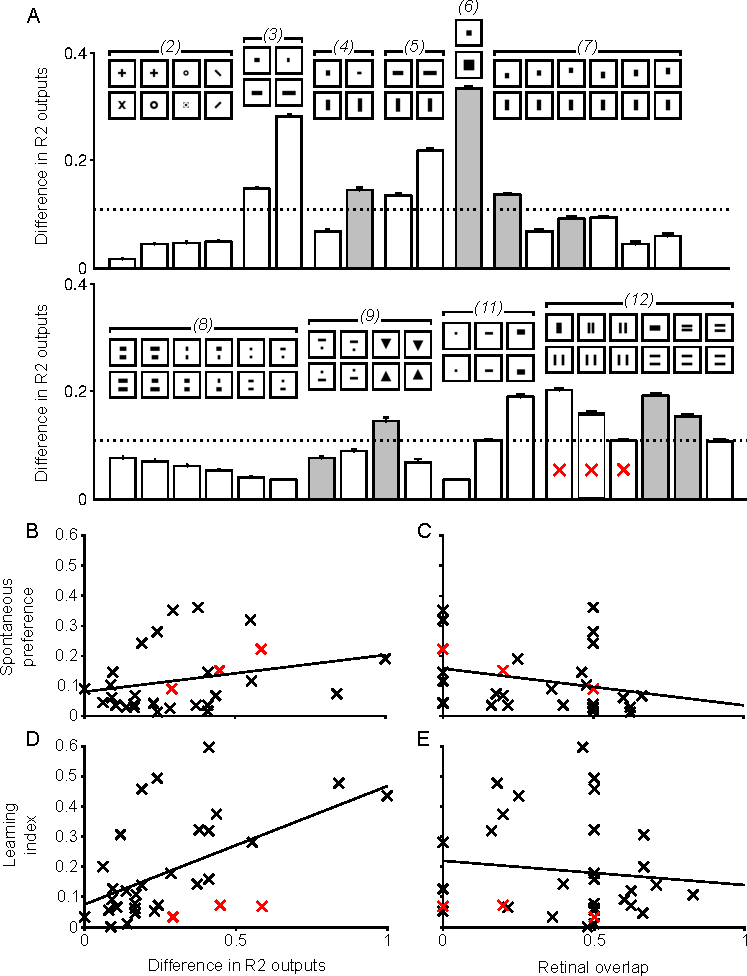
\includegraphics{figures/pattern}
\caption{ PRG 31/7/15 Outputs of simulated R2 populations for published pattern pairs.
A, B: As per the methond in Figure 1 we calculate the \ac{rms} difference in R2 activity for simulated flies viewing each pattern in a pattern array. The patterns tested here are drawn from \protect\cite{Ernst1999} and are grouped together according to the figures in which they appear in that work.
The corresponding figure numbers are shown in parentheses.
All pattern pairs for which the significance of `learning preference' ($\overline{\mathrm{DCP}}$) was given are included. Grey bars indicate that the $\overline{\mathrm{DCP}}$ for the pattern was significant ($p<.05$).
A higher score indicates a greater in R2 activity and thus that the pattern pair was more discriminable by the population code from the simulated R2 cells.
C-F: Scatter plots of \ac{rms} difference in R2 output and simple retinal overlap for pattern pairs \emph{vs} learning index ($\overline{\mathrm{DCP}}$) and spontaneous preference for the same pattern pairs from Ernst and Heisenberg \protect\cite{Ernst1999}.
The correlations for \ac{rms} difference in R2 output was found to be significant for spontaneous preference (C, Spearman's rank, $n=34, \rho=.615, p<.005$) and learning index (D, $n=34, xxxx, p=xxxx$). There was no correlation between Retinotopic overlap and spontaneous preference(D, $n=34, \rho= -0.215, p=\mathrm{n.s.}$) or learning index (E, xxx, xxx, xxx, p=xxx).
}
\label{fig:pattern}
\end{figure}
